\documentclass[12pt]{article}
\usepackage[latin1]{inputenc}
\usepackage{geometry} % see geometry.pdf on how to lay out the page. There's lots.
\geometry{a4paper} % or letter or a5paper or ... etc
% \geometry{landscape} % rotated page geometry
\usepackage{amsfonts}

\usepackage{amsthm}
\newtheorem{theorem}{Theorem}

\usepackage{graphicx}
\usepackage{acronym}
\usepackage{pgfplots}
\pgfplotsset{compat=1.8}
\usepgfplotslibrary{statistics}

\usepackage{algpseudocode}
\usepackage{algorithm}

\title{Selection of Polynomial Features by Genetic Algorithms}
\author{Francisco Coelho \and Jo�o Neto}
\date{[{\sc draft} \today]} % delete this line to display the current date

\newcommand{\sample}[1]{\ensuremath{^{\left(#1\right)}}}

\acrodef{GA}{Genetic algorithms}
\acrodef{rmse}{root-mean-square error}
\acrodef{GAPoly}[{\sc GAPoly}]{Genetic Algorithms for Polynomials}

%%% BEGIN DOCUMENT
\begin{document}


\maketitle
\begin{abstract}
Many applications require models that have no acceptable linear approximation and many nonlinear models are defined by polynomials. The use of genetic algorithms to find polynomial models is decades old but still poses challenges due to the complexity of the search and different definitions of optimal solution.

This paper describes a two-step method that uses genetic algorithms and linear regression to find empirical polynomial regressions. Experiments on common datasets show that, discounting the training computational effort, this method is quite competitive.
\end{abstract}

\section{Introduction}

With notable exceptions (\emph{e.g.} neural networks) machine learning regression techniques are based on linear models. The linearity assumption has many advantages including reduced computational complexity and strong theoretical framework. However nonlinearity is unavoidable in many application scenarios, specially those with phase transitions or feedback loops, so common in ecology, cybernetics, robotics and other areas.

Polynomials, one of the most studied subjects in mathematics, generalize li\-ne\-ar functions and define, perhaps, the simplest and most used nonlinear models. Applications include colorimetric calibration \cite{mendes2005adaptive}, explicit formulae for turbulent pipe flows \cite{davidson1999method}, computational linguistics \cite{sanchez2009obtaining} and more recently, analytical techniques for cultural heritage materials \cite{csefalvayova2010use}, liquid epoxy molding process \cite{chan2011modeling}, B-spline surface reconstruction \cite{galvez2012iterative}, product design \cite{chan2012development} or forecasting cyanotoxins presence in water reservoirs \cite{garcia2013hybrid}. This not only illustrates the wide spectrum of applications but, additionally, work in each one of these polynomial models uses, at some point, a genetic algorithm.

\ac{GA} where, arguably, one the hottest topics of research in the recent decades and with good reason since they outline an optimization scheme easy to conceptualize and with very broad application. If a nonlinear (or otherwise) model requires parameterization, \acp{GA} provide a simple and often effective approach to search for locally optimal parameters. Research related to genetic algorithms abound and spans from the 1950s seminal work of Nils Aall Barricelli \cite{barricelli1962numerical} in the Institute for Advanced Study of Princeton to today's principal area of study for thousands of researchers, covered in hundreds of conferences, workshops and other meetings. Perhaps the key impulse to \acp{GA} come from John Holland's work and his book ``Adaptation in Natural and Artificial Systems'' \cite{holland1975adaptation}.  

One interesting take on genetic algorithms, named \emph{genetic programming} by John Koza \cite{koza1992genetic}, proposed the use of \acp{GA} to search the syntactic structure of complex functions. This syntatic structure search is keen to the central ideas of deep learning \cite{bengio2013representation, bengio2009learning}, the subarea of machine learning actually producing the most promising results (\emph{e.g.} \cite{tarlowstochastic}). It is also related to the work presented in this paper in the sense that, unlike linear models that have a simple structure, $y=\sum_i \beta_i x_i$, nonlinear (in particular polynomial) models pose an additional ``structure" search problem.

The idea of using \acp{GA} to find a polynomial regression is not new \cite{maertens2006genetic, yu2008optimal, wu2009novel} but still generates original research \cite{hofwing2011optimal, cetisli2011polynomial}. In line with that research this work describes a general method to find a polynomial regression of a given dataset. The optimal regression minimises a cost function that accounts for both the \ac{rmse} and a regularization factor to avoid over-fitting. 

%A method that produces \emph{adequate} models from observed complex data has many uses. For example by a scientist to better understand the source of the data or by an autonomous agents adapting to the environment.  

It turns out that, discarding the computational cost of training, the polynomial regression method presented here, \ac{GAPoly}, provides a quite competitive regression method. Indeed, it is only systematically out-performed by random forests, an \emph{ensemble} method.

The remainder of this paper is organized as usual: the next section describes the details of our method and is followed by a presentation of some performance results. The last section draws some conclusions and points future research tasks.


\section{Genetic Algorithms for Polynomials}

This section is dedicated to describe an algorithm to find a polynomial regression from a given dataset. It starts with a brief introduction and description of the algorithm and proceeds into core details as the encoding used to represent individual polynomial instances in the \ac{GA} populations and the regularization of the cost function.

A usual representation of polynomials is
$$
p\left( x_1, \ldots, x_k\right) = \sum_i \theta_i m_i
$$
where each $m_i$ is a monomial, $m_i = \prod_{j} x_j^{\alpha_{ij}}$, the exponents are non-negative integers, $\alpha_{ij}\in\mathbb{N}_0$, and the coefficients are real valued, $\theta_i \in \mathbb{R}$. For example $p\left( x_1, x_2, x_3 \right) = 2 x_1 + x_2 x_3 + \frac{1}{2} x_1^2 x_3$ has monomials $m_1 = x_1, m_2 = x_2 x_3$ and $m_3 = x_1^2 x_3$ coefficients $\theta_1 = 2, \theta_2 = 1$ and $\theta_3 = 1/2$ and exponents $\alpha_{1,1} = 1, \alpha_{2,2}=1, \alpha_{2,3} = 1, \alpha_{3,1} = 2, \alpha_{3,3} = 1$ and all other $\alpha_{ij} = 0$. The exponents alone are a matrix that defines the monomial structure of the polynomial, $A = \left[\alpha_{ij}\right]$. For the example above
$$
A = \left[ 
\begin{array}{ccc}
1 & 0 & 0 \\
0 & 1 & 1 \\
2 & 0 & 1
\end{array}
\right] \sim 
\left[ 
\begin{array}{ccc}
x_1 \\
x_2 x_3 \\
x_1^2 x_3
\end{array}
\right]
$$
where each row defines a monomial and each column represents a variable. Changing the order of the rows doesn't change the polynomial whereas changing the order of the columns corresponds to changing the respective variables.
%Notice that if we interpret matrix $A$ as a single column of monomials and set the coefficients $T = \left[ \begin{array}{ccc} 2 & 1 & \frac{1}{2} \end{array} \right ]$ then
%$$
%p\left( x_1, x_2, x_3 \right) = TA = \left[ \begin{array}{ccc} 2 & 1 & \frac{1}{2} \end{array} \right ]\left[ 
%\begin{array}{ccc}
%x_1 \\
%x_2 x_3 \\
%x_1^2 x_3
%\end{array}
%\right].
%$$

This representation of polynomials makes the problem of structure search very clear: except for the trivial cases, the number of possible monomials given $n$ variables and a maximum joint degree $d$ grows exponentialy with either $n$ or $d$. But more importantly, the polynomial regression problem can be naturally split into two subproblems:
%
\begin{enumerate}
\item for a given set of monomials $m_1, \ldots, m_R$, find the regression coefficients $\theta_1,\ldots,\theta_R$ that minimize the \ac{rmse} on a given dataset;

\item find the fittest set of monomials, \emph{i.e.} the polynomial that minimizes the \ac{rmse} on the same dataset;
\end{enumerate}
%
More precisely, concerning the first problem, let $\mathcal{D}$ be a dataset with $N$ observations of variables $Y, X_1,\ldots,X_n$ and $\mathcal{M} = \left\lbrace m_1,\ldots, m_R\right\rbrace$ a set of $R$ monomial expressions over $X_1,\ldots,X_n$. Define the hypothesis\footnote{The expression $m|_{X=x}$ reads ``\emph{replace all instances of $X$ by $x$ in $m$}''.}
%
\begin{eqnarray*}
h_{\Theta,\mathcal{M}}\left(x_1,\ldots,x_n\right) &=& \sum_{j = 1}^R \theta_j m_j|_{X_i=x_i,\forall 1 \leq i \leq n}
\end{eqnarray*}
%
and let the cost
%
\begin{eqnarray}
J\left(\Theta;\mathcal{M},\mathcal{D}\right) &=& \sqrt{\frac{1}{N}\sum_{i=1}^N \left( y\sample{i} - h_{\Theta,\mathcal{M}}\left( x_1\sample{i},\ldots,x_n\sample{i} \right) \right)^2 }\label{eq:rmse}
\end{eqnarray}
%
be the usual \acf{rmse} function. Now the first problem can be stated as:
%
\begin{quote}
Given a dataset $\mathcal{D}$ and a set of monomials $\mathcal{M}$, find parameters $\Theta$ that minimize $J\left(\Theta;\mathcal{M},\mathcal{D}\right)$.
\end{quote}
%
It turns out that this problem can be solved as a usual linear regression problem by expanding $\mathcal{D}$ with columns that replicate the monomials in $\mathcal{M}$.

The second problem is treated in the \ac{GA} setting: Let $\mathcal{D}$ be a dataset as above and $\mathcal{P}$ a set of polynomials. For each polynomial $p\in \mathcal{P}$ let $\mathcal{M}_p$ be the set of monomials in $p$ (without the coefficients) and compute the fitness
%
\begin{eqnarray*}
\phi_p &=& \min_\Theta J\left(\Theta;\mathcal{M}_p,\mathcal{D}\right)
\end{eqnarray*}
%
by solving the first problem. With a fitness of every instance, a \ac{GA} will apply genetic operators (usually mutation and crossover) to evolve the population $\mathcal{P}$ until a reasonable approximation of a local minimum is found. 
%
\begin{algorithm}[htb]
\begin{algorithmic}
\Function{GAPoly}{$D,pop_0,\epsilon$}
	\State $pop \gets pop_0;\: err \gets 1.0+\epsilon$
	\While{$err > \epsilon$}
		\State $pop \gets \Call{IterateGA}{pop}$\Comment{Build next generation}
		\State $pop \gets \Call{Sort}{pop, key = \textsc{Lm.rmse}}$\Comment{Sort by \ac{rmse} of linear regression}
		\State $err \gets \textsc{rmse}\left(\Call{First}{pop}\right)$
	\EndWhile
	\State\Return $\Call{First}{pop}$
\EndFunction
\end{algorithmic}
\caption{\ac{GAPoly} uses linear regression to find monomial coefficients that minimize the \ac{rmse} over a dataset and \acp{GA} to explore the space of polynomials. At exit the \ac{rmse} of the fittest instance is bounded by $\epsilon$.}\label{alg:gapoly}
\end{algorithm} 
%
\begin{theorem}
The composition of \acp{GA} with linear regression, as defined in Algorithm \ref{alg:gapoly}, converges to a polynomial that is a local minimum of the \ac{rmse} function, encapsulated in the fitness function $J$.
\end{theorem}
%
\begin{proof}
It follows from the properties of \acp{GA} and linear regression.
\end{proof}
%
Subsection \ref{subs:polynomial.encoding} details of the encoding of individual polynomial instances as chromosomes and other parameters of the \ac{GA} implementation used. The regularization of the cost function is discussed in subsection \ref{subs:cost.function}.
\subsection{Polinomial Encoding}\label{subs:polynomial.encoding}

The chromosome coding will as follow:
\begin{enumerate}
\item an initial segment detailing which monomials are active (the 1st monomial is always active), these are represented in unary description
\item the chromosome is split into $m$ sets of bits of equal size 
  (a monomial)
\item each monomial is split into $n$ sets of $d$ size each, i.e., a variable
\item for each variable, the remaining bits give the binary description of the variable degree, i.e., the maximum exponent is given by $2^d-1$
\end{enumerate}

Eg: consider polynomial $x_1^3 x_3 + x_3^7 + x_1 x_2$ with $m = 4, n = 3$ and $d=3$. One possible encoding would be:
$$110 - 011,000,001~~;~~000,000,111~~;~~001,001,000~~;~~110,010,101$$

(for reading purposes the semicolons separate monomials, the commas separate variables)

The first $3$ bits inform that the second and third monomials are active while the fourth is not (as said, the first monomial is always active). This last monomial does not enter neither in the polynomial regression nor in the fitness evaluation. However, it acts as a kind of junk DNA, becoming active when the third bit of the entire sequence flips from 0 to 1.

Let's interpret the first monomial description, $011,000,001$. It is divided by three since $n=3$. The first triple $011$ is the binary description of the exponent of variable $x_1$ which is 3, so the first monomial includes $x_1^3$. The second triple, $000$, means that $x_2$ is not part of the monomial. The third triple $001$ says that variable $x_3$ has exponent $1$, so the first monomial consists of $x_1^3 x_3$. All the remaining sets of $9$ bits are interpreted the same way and we get the previous polynomial.

Notice that all binary descriptions give rise to valid polynomials. However, if the coding consists of entirely zeros, by convention, it describes polynomial $x_1$. This has to do with the execution of the polynomial regression that would fail if we interpret it as the zero polynomial. Anyway, for progressive larger  binary descriptions, the chances of getting this zero description decrease exponentially, so it does not impact in any meaningful way in the algorithm's performance.


\subsection{Cost Function}\label{subs:cost.function}

The polynomial fitness considered so far is based on the ability to predict the test set after the polynomial regression has found the appropriate coefficients $\theta_i$ for each one of the polynomial's monomials $m_i$.

This fitness function tends to prefer more complex polynomials, namely in the number of monomials which provides the regression algorithm for more fitting possibilities. One way to balance this is to provide a regularization term into the fitness function. Our proposal is to include a multiplicative factor into the fitness function proportional to the number of monomials. Thus, the fitness function becomes,

$$
J_{fit}\left( \Theta; D \right) = \lambda^{m} \sqrt{ \frac{1}{n} \sum_{i=1}^n \left( y^{(i)} - h_{\Theta}\left(x_1^{(i)}, \ldots, x_m^{(i)}\right) \right)^2 }
$$

where $m$ is the number of monomials the polynomial has. A $\lambda$ greater than one punishes polynomials with more monomials.

Somewhat unexpectedly after some experiences it was found that lower values for $\lambda$ sometimes provide better, even if marginal, results. Figure~\ref{Abalone_dataset_lambdas} shows results for the Abalone dataset with five runs for each $\lambda$ (cf. Experimental Results includes information about these datasets).

\begin{figure}[htb]\begin{center}
\begin{tikzpicture}
\begin{axis}[width=\textwidth,height=6cm,
	boxplot/draw direction=y,
	xtick={1,2,3,4,5,6,7,8,9,10,11,12,13},
	xticklabels={0.70, 0.75, 0.80, 0.85, 0.90, 0.95, 1.00, 1.05, 1.10, 1.15, 1.20, 1.25, 1.30},
	xlabel={regularisation exponent ($\lambda$)},
	ymin=2.0,
	ymax=3.0,
	ylabel={Error distribution (\ac{rmse})},
	title={Error distribution by regularisation exponent (\textbf{Abalone dataset})},
	mark options={scale=0.5},
	]
	\addplot[only marks, mark=o,color=black] table [x expr=1+0.2*rand,y index=0] {data/figure1.dat};
	\addplot[only marks, mark=o,color=black] table [x expr=2+0.2*rand,y index=1] {data/figure1.dat};		
	\addplot[only marks, mark=o,color=black] table [x expr=3+0.2*rand,y index=2] {data/figure1.dat};
	\addplot[only marks, mark=o,color=black] table [x expr=4+0.2*rand,y index=3] {data/figure1.dat};
	\addplot[only marks, mark=o,color=black] table [x expr=5+0.2*rand,y index=4] {data/figure1.dat};
	\addplot[only marks, mark=o,color=black] table [x expr=6+0.2*rand,y index=5] {data/figure1.dat};
	\addplot[only marks, mark=o,color=black] table [x expr=7+0.2*rand,y index=6] {data/figure1.dat};
	\addplot[only marks, mark=o,color=black] table [x expr=8+0.2*rand,y index=7] {data/figure1.dat};
	\addplot[only marks, mark=o,color=black] table [x expr=9+0.2*rand,y index=8] {data/figure1.dat};
	\addplot[only marks, mark=o,color=black] table [x expr=10+0.2*rand,y index=9] {data/figure1.dat};
	\addplot[only marks, mark=o,color=black] table [x expr=11+0.2*rand,y index=10] {data/figure1.dat};
	\addplot[only marks, mark=o,color=black] table [x expr=12+0.2*rand,y index=11] {data/figure1.dat};
	\addplot[only marks, mark=o,color=black] table [x expr=13+0.2*rand,y index=12] {data/figure1.dat};
	
	\pgfplotsset{boxplot/every box/.append style={fill=gray!50!white}}
	\addplot[boxplot] table [y index=0] {data/figure1.dat};
	\addplot[boxplot] table [y index=1] {data/figure1.dat};
	\addplot[boxplot] table [y index=2] {data/figure1.dat};
	\addplot[boxplot] table [y index=3] {data/figure1.dat};
	\addplot[boxplot] table [y index=4] {data/figure1.dat};
	\addplot[boxplot] table [y index=5] {data/figure1.dat};
	\addplot[boxplot] table [y index=6] {data/figure1.dat};
	\addplot[boxplot] table [y index=7] {data/figure1.dat};		
	\addplot[boxplot] table [y index=8] {data/figure1.dat};
	\addplot[boxplot] table [y index=9] {data/figure1.dat};
	\addplot[boxplot] table [y index=10] {data/figure1.dat};
	\addplot[boxplot] table [y index=11] {data/figure1.dat};
	\addplot[boxplot] table [y index=12] {data/figure1.dat};

\end{axis}
\end{tikzpicture}
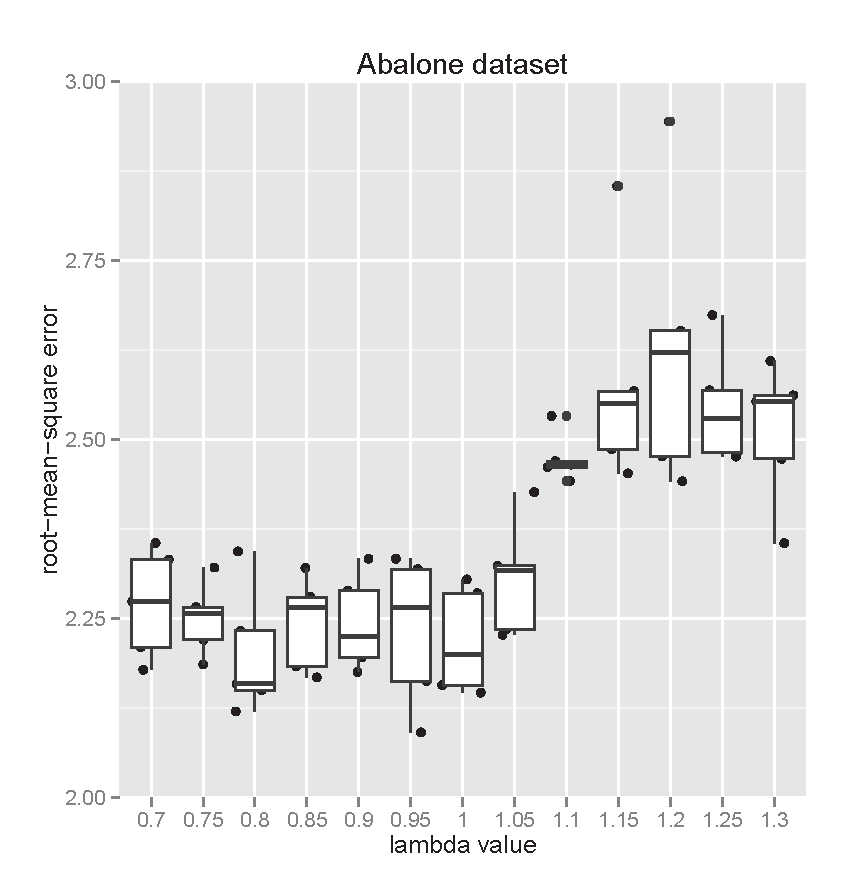
\includegraphics[height=6cm,width=\textwidth,angle=0]{figures/Abalone_dataset_lambdas.eps}

\caption{Fitness progress for the Abalone dataset.}\label{Abalone_dataset_lambdas}

\end{center}\end{figure}

%\begin{figure}[htb]
%	\begin{center}
%		\includegraphics[height=6cm,width=10cm,angle=0]
%			{figures/Abalone_dataset_lambdas.eps}
%		\caption{fitness progress for Abalone dataset}
%		\label{Abalone_dataset_lambdas}
%	\end{center}
%\end{figure}

Figure~\ref{Auto-Mpg_dataset_lambdas} presents regularization results for the Auto-MPG dataset:

\begin{figure}[htb]
	\begin{center}
		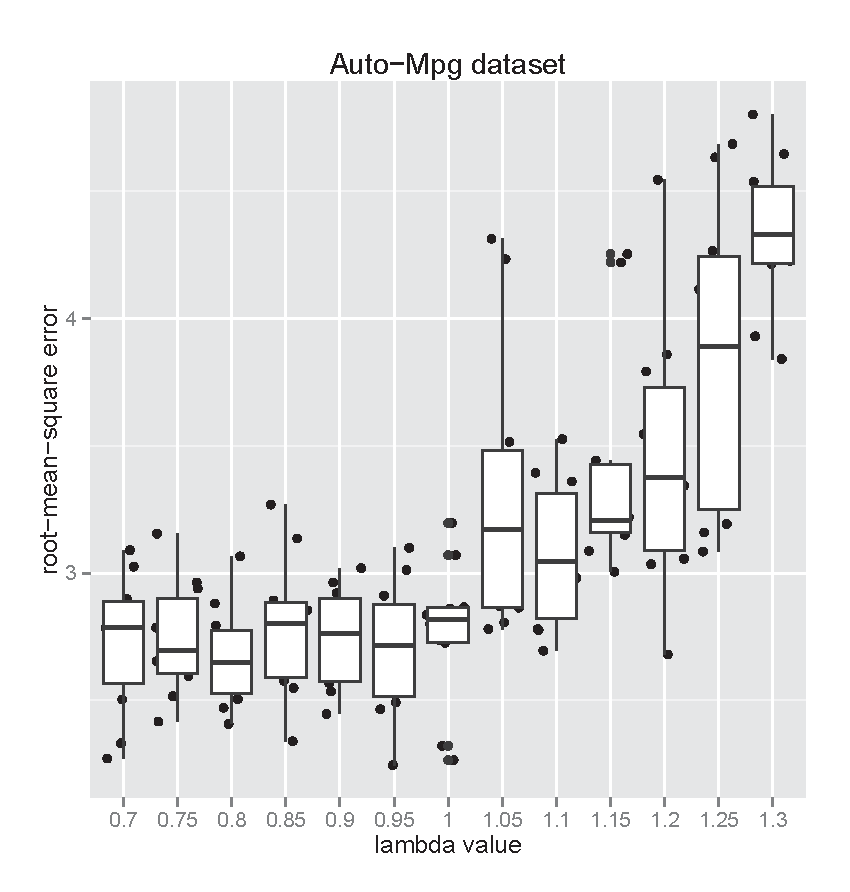
\includegraphics[height=6cm,width=10cm,angle=0]
			{figures/Auto-Mpg_dataset_lambdas.eps}
		\caption{fitness progress for Abalone dataset}
		\label{Auto-Mpg_dataset_lambdas}
	\end{center}
\end{figure}

The typical inflection point is around $\lambda = 0.8$. We'll use the regularisation parameter with this value.

\subsection{Genetic Operators}

\emph{Define the genetic operators}

\subsection{Other Search Parameters}

\emph{Explain the remaining search parameters}

\section{Experimental Results}

\begin{itemize}
\item Measured quantities
	
	\begin{itemize}

	\item error
	\item number of iterations to convergence
	\item memory usage
	\item F1, ROC, ?  
	
	\end{itemize}

\item Selection of datasets and regression algorithms
\item Summary Figures and Numeric results
\end{itemize}
These results were found using R's programming language~\cite{R}.

To compare this paper's algorithm we applied the exact same train and test samples with other learning algorithms, namely: Linear Regression, Support Vector Machines~\cite{Meyer12}, Regression Trees~\cite{Therneau13}, Conditional Inference Trees~\cite{Hothorn06, Strobl07, Strobl08} and Random Forests~\cite{Liaw02}

In order to train and test the performance of \ac{GAPoly} it was used several datasets (see below). For each dataset, we selected 70\% for training purposes and the remaining observations to make the test set in order to compute the estimated \ac{rmse}. To achieve more robust results, for most datasets there were 25 runs, each one with different samples for the train and test sets. For the datasets with attribute values of different magnitudes, a preliminary scaling was executed. The results below are boxplots for the test set error predictions over these different runs.

\textbf{Artificial}: this is an artificial dataset with four numeric features, $x_1, \ldots x_4$, where $x_1,x_3$ are outcomes from Poisson random variables, and $x_2,x_4$ from Normal random variables. The dependent variable $y$ is given by expression $x_2x_4^2 + x_1^2x_3 + 5$. The dataset includes 50 observations. 

\begin{figure}[htb]
	\begin{center}
		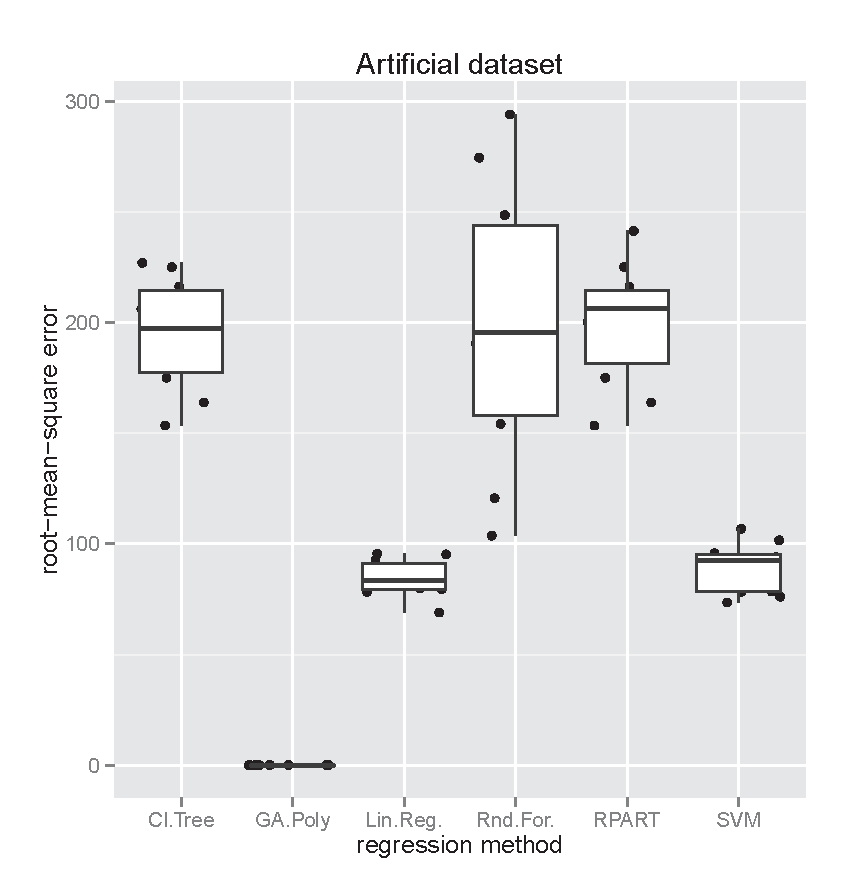
\includegraphics[height=6cm,width=10cm,angle=0]
			{figures/artificial_dataset1_lambda1_0.eps}
		\caption{results for Artificial dataset}
		\label{artificial_dataset1_lambda1.0}
	\end{center}
\end{figure}

This dataset was used in order to verify if \ac{GAPoly} was able to find the polynomial relation, which the algorithm did (cf. figure~\ref{artificial_dataset1_lambda1.0}). In this case, all runs used a population of 100 with 50 iterations for each run.

In the next datasets, the population has size 250 with 100 iterations for each run.

\textbf{Housing}: This data set concerns the task of predicting housing values in areas of Boston. There are 13 continuous attributes and the dependent variable is the median value of owner-occupied homes in \$1000's\footnote{This and the remaining regression datasets were selected from Luis Torgo's data repository, http://www.dcc.fc.up.pt/~ltorgo/Regression/DataSets.html. Most of these set originally come from UCI ML repository, http://archive.ics.uci.edu/ml/}. There are 506 observations. Figure~\ref{Housing_dataset_lambda0.8_25runs} presents the results for this dataset.

\begin{figure}[htb]
	\begin{center}
		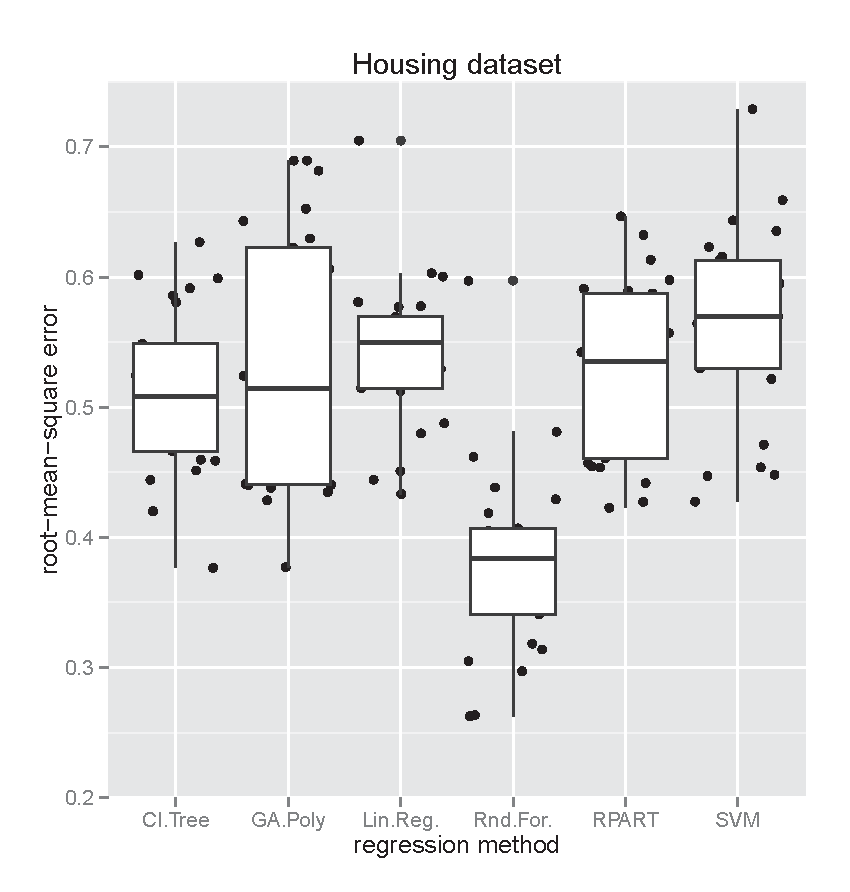
\includegraphics[height=6cm,width=10cm,angle=0]
			{figures/Housing_dataset_lambda0_8_25runs.eps}
		\caption{results for Boston Housing dataset}
		\label{Housing_dataset_lambda0.8_25runs}
	\end{center}
\end{figure}

Just as an example of the model the \ac{GAPoly} algorithm outputs: in this dataset the best polynomial, with a \ac{rmse} of 0.38 for the test set, was the following:

$$y = -0.12 x_6 x_9^4 + 0.78 x_6 - 0.4 x_9^2 x_{13} + 0.17 x_{13}^2 - 0.044$$

where the attributes mean:
$x_6$, RM average number of rooms per dwelling;
$x_9$, RAD index of accessibility to radial highways;
$x_{13}$, Lower status of the population.

\textbf{Abalone}: This dataset can be used to predict the age of a abalone shell using the given 8 numeric attributes concerning several physical measurements. There are 4177 observations. Figure~\ref{Abalone_dataset_lambda0.8_25runs} presents the results for this dataset.

\begin{figure}[htb]
	\begin{center}
		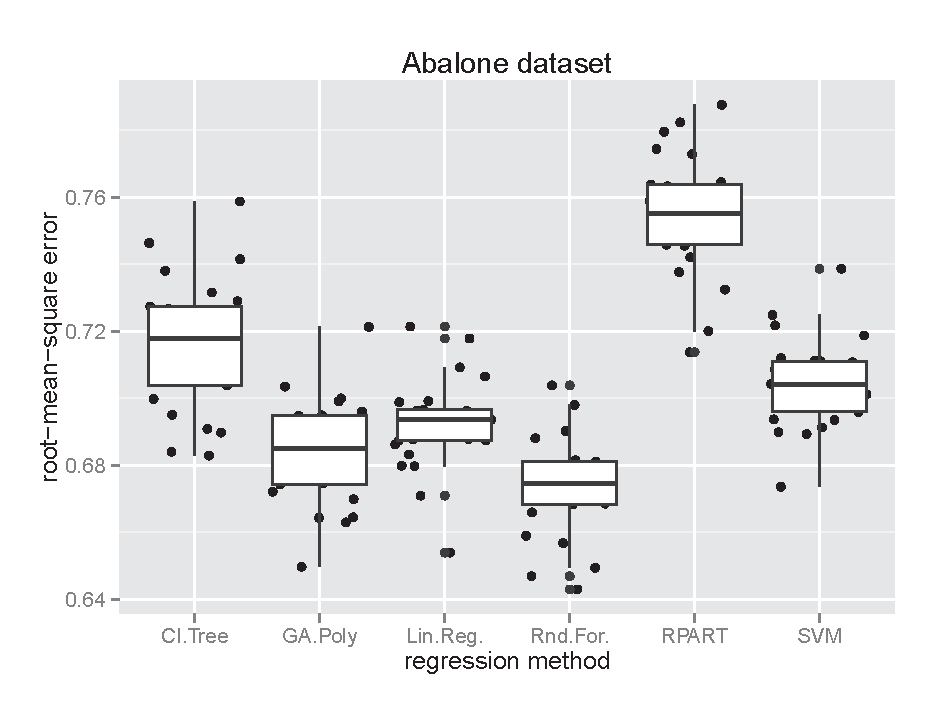
\includegraphics[height=6cm,width=10cm,angle=0]
			{figures/Abalone_dataset_lambda0_8_25runs.eps}
		\caption{results for Abalone dataset}
		\label{Abalone_dataset_lambda0.8_25runs}
	\end{center}
\end{figure}

% best polynomial, rsme 0.65
% $$y = 0.52 s_1^2 x_5 - 0.13 x_2 x_8 -0.75 x_1^2 x_6 + 0.78 x_8 + 0.18 $$

\textbf{Auto-MPG}: This dataset is used to predict fuel consumption in miles per gallon, based on two discrete and five continuous attributes. There are 398 observations. Figure~\ref{Auto-Mpg_dataset_lambda0.8_25runs} presents the results for this dataset.

\begin{figure}[htb]
	\begin{center}
		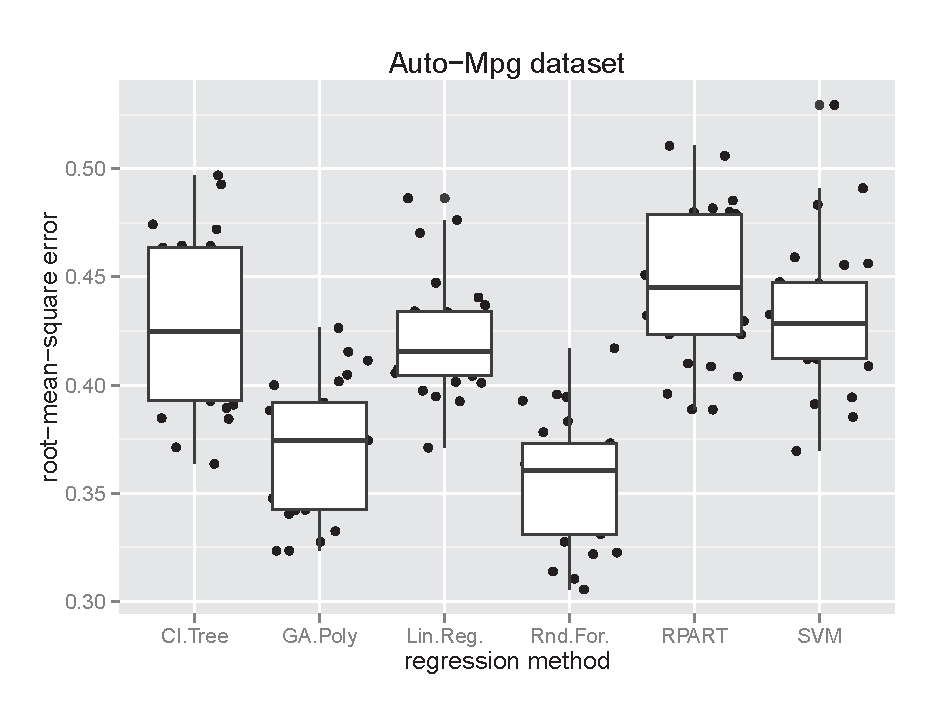
\includegraphics[height=6cm,width=10cm,angle=0]
			{figures/Auto-Mpg_dataset_lambda0_8_25runs.eps}
		\caption{results for Auto-MPG dataset}
		\label{Auto-Mpg_dataset_lambda0.8_25runs}
	\end{center}
\end{figure}

% best polynomial, \ac{rmse} 0.32
%$$ y = 0.4 x_6 + 0.02 x_5^3 x_6 - 0.85 x_4 + 0.23 x_4^2 - 0.26 $$

\textbf{Kinematics}: This dataset is concerned with the realistic simulation of the forward kinematics of an 8 link robot arm. The task is to predict the distance of the end-effector from a target using 8 continuous attributes. There are 8192 observations. Figure~\ref{Kinematics300_lambda0.8_25runs} presents the results for this dataset.

\begin{figure}[htb]
	\begin{center}
		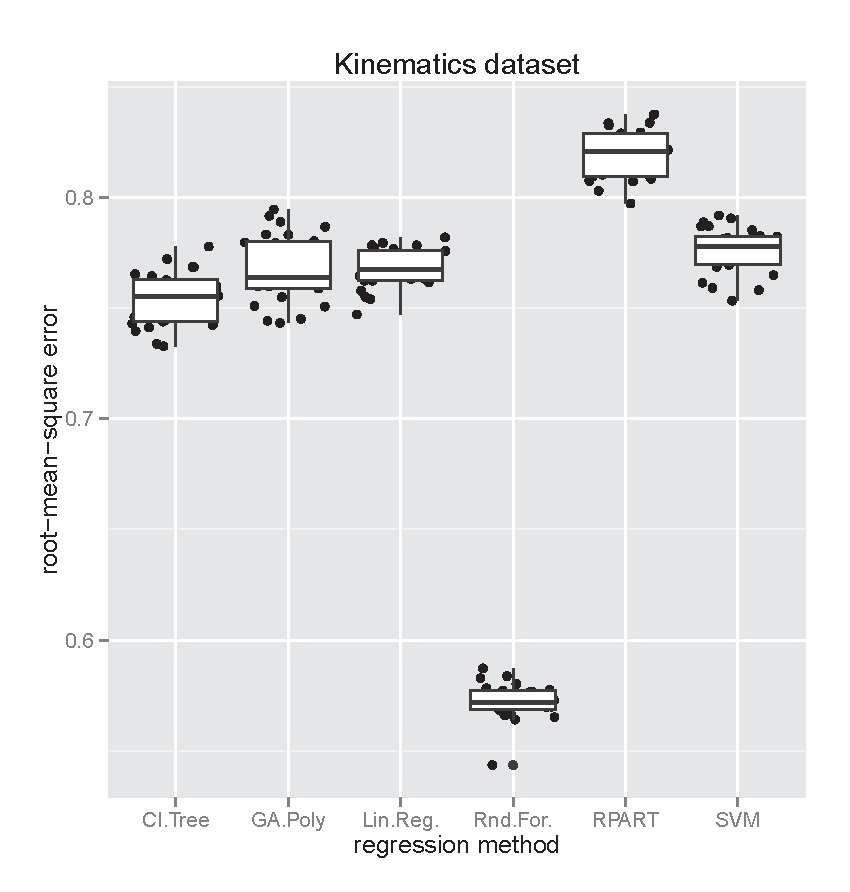
\includegraphics[height=6cm,width=10cm,angle=0]
			{figures/Kinematics300_lambda0_8_25runs.eps}
		\caption{results for Kinematics dataset}
		\label{Kinematics300_lambda0.8_25runs}
	\end{center}
\end{figure}

% best polynomial, \ac{rmse} 0.74
% $$ y = 0.24 x_5 - 0.23 x_5 x_6 x_7 - 0.19 x_4 x_7 - 0.5 x_3 $$

\subsection{Convergence speed}

The \ac{GA} quickly proceeds in the first 50 to 100 generations to reasonable error rates. Then, it proceeds slower achieving best solutions with marginal error reduction. Since the entire learning process takes some time, in the current R implementation\footnote{The processing time can probably be speeded by one to two orders in magnitude if the process is implemented in a low level programming language like C++. However, speed optimisation was not the focus of this article}, placing a limit between 50 to 100 generations already achieves good results, relative to higher iteration values. Figure~\ref{Abalone_fitnessProgress} shows a typical error evolution for the dataset Abalone given two different values for $\lambda$.

\begin{figure}[htb]
	\begin{center}
		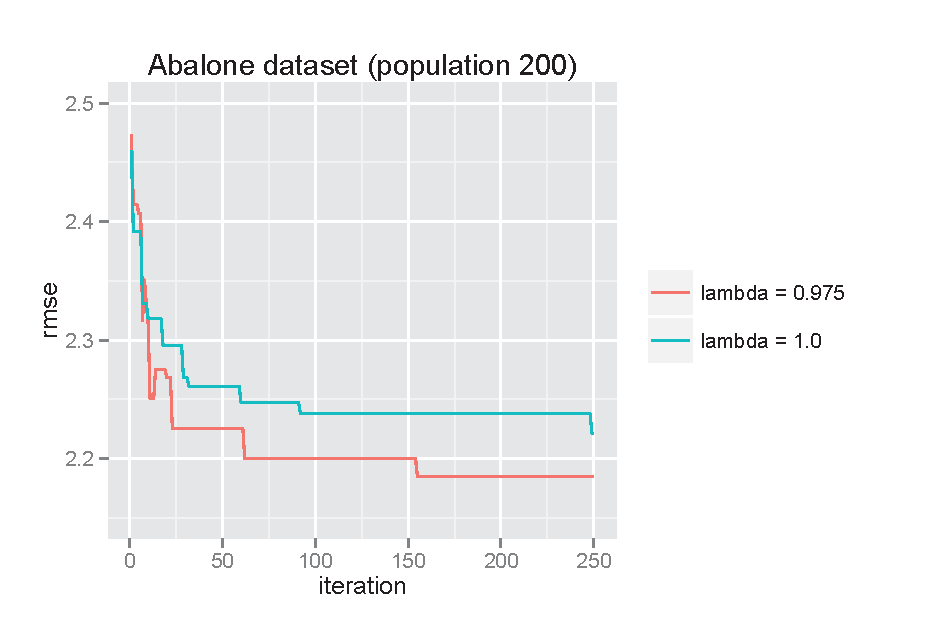
\includegraphics[height=6cm,width=10cm,angle=0]
			{figures/Abalone_fitnessProgress.eps}
		\caption{fitness progress for Abalone dataset}
		\label{Abalone_fitnessProgress}
	\end{center}
\end{figure}



\section{Conclusion}



\subsection{Discussion}

The proposed method has competitive results comparing with some well-known regression methods. Only Random Forest outperforms \ac{GAPoly} systematically (it outperforms all the others) except in the Auto-MPG test and, of course, in the artificial dataset that uses a straightforward polynomial relation. 

\section{Bibliography}

\bibliographystyle{plain}
\bibliography{fullbib}

\end{document}